\documentclass[a4paper, 12pt]{article}%тип документа

%отступы
\usepackage[left=1cm,right=1cm,top=1cm,bottom=2cm,bindingoffset=0cm]{geometry}

%Русский язык
\usepackage[T2A]{fontenc} %кодировка
\usepackage[utf8]{inputenc} %кодировка исходного кода
\usepackage[english,russian]{babel} %локализация и переносы

%Вставка картинок
\usepackage{graphicx}
\graphicspath{{pictures/}}
\DeclareGraphicsExtensions{.pdf,.png,.jpg}

%Графики
\usepackage{pgfplots}
\pgfplotsset{compat=1.9}

%Математика
\usepackage{amsmath, amsfonts, amssymb, amsthm, mathtools}

%Заголовок
\author{Валеев Рауф Раушанович \\
группа 825}
\title{\textbf{Работа 1.1.6 \\
Изучение электронного осцилогрофа}}

\begin{document}
\maketitle
\newpage
\begin{enumerate}
\item	
	\textbf{Подготовка к работе.}
	\begin{enumerate}
	\item Блок горизонтальной развертки (HORIZONTAL): ручка POSITION -  в среднем положении; кнопка х10 MAG - отжата; ручка SWP.VAR - в крайнем правом положении;
	\item Блок вертикального отклонения (VERTIСAL): ручки POSITION — в среднем положении; внешние ручки VOLTS/DIV обоих каналов в положении 5 V/дел, а внутренние — утоплены; тумблеры AC–GND–DC обоих каналов — в положении GND (отключены); кнопки ALT/CHOP и INV CH 2 — отжаты.
	\item Блок синхронизации (TRIGGER): TRIG.ALT — отжата, LEVEL — в среднем положении; переключатель MODE — в положении AUTO; SLOPE — отжата.
	\item Включиаем осциллограф в сеть. Ставим ручку развертки
TIME/DIV в положение X–Y. На экране появится точка. Ручками POSITION располагаем точку в центре экрана осциллографа. Регулируем яркость и четкость изображения точки ручками INTEN и FOCUS — размер и яркость точки должны быть минимально возможными, при условии, что точка хорошо видна на экране. После регулировки включите внутреннюю развертку осциллографа, установив ручку TIME/DIV в положение 2 ms.	
	\end{enumerate}
\item 
	\textbf{Наблюдение периодического сигнала.} \\ От генратора и измерение его частоты. Получаем на экране устойчивую картину периодического синусоидального сигнала, подаваемого с генератора, и с помощью горизонтальной шкалы экрана осцилогрофа проводим измерение периода и частоты сигнала. 
	\begin{enumerate}
	\item Настраиваем подключенный к каналу CH2 звуковой генератор на синусоидальный сигнал с частотой $f\approx 1 kHz$. Переключаем тумблер MODE блока VERTICAL и тумблер SOURCE блока TRIGGER в положение CH2(Y). Устанавливаем режим канала CH2(Y) на открытый вход (DC).
	\item Получаем на осциллографе устойчивую картину колебаний. Используя ручки VOLTS/DIV (вольт/деление) для регулировки масштаба по вертикали, TIME/DIV (время/деление) — для регулировки масштаба по горизонтали, ручки POSITION для смещения картины как целого. Используя ручку LEVEL (уровень запуска развертки) для получения стационарной картины. При необходимости переключаем режим синхронизации тумблером MODE блока TRIGGER в положения AUTO (автоматический запуск развертки) или NORM (режим ожидания).
	\item Измеряем период колебаний $T$ наблюдаемого сигнала с учетом масштаба. Расчитываем его частоту $f$. Оценим погрешность $\delta F$ и $\delta T$. Сравниваем с показаниями встроенного в генератор частотометра $f_{\text{ЗГ}}$ или с положением ручек регулировки генератора. Повторяем для 3-5 разлчиных частот.
	\begin{figure} [h]
		\center{
	\begin{tabular}{|c|c|c|c|c|c|c|c|}
	\hline
	$f1,kHz$&$T$, дел&дел&$T, c$&$f, kHz$&$\delta f, kHz$&$\delta T, c$&$f1-f, kHz$ \\
	\hline
	1,1&1&0,001&0,001&1&0,1&$10^{-4}$&0,1\\
	\hline
10,822&1,87&$50*10^{-6}$&$93,3*10^{-6}$&11&0,6&$5*10^{-6}$&0,178\\
\hline
110,84&0,9&$10^{-5}$&$9*10^{-6}$&111&6&$5*10^{-7}$&0,16\\
\hline
1260&1,6&$5*10^{-7}$&$8*10^{-7}$&1250&80&$5*10^{-8}$&10\\
\hline
	\end{tabular}
		}
	\end{figure}
	\end{enumerate}
	\item \textbf{Измерение амплитуды сигнала.} \\С помощью вертикальной шкалы экрана осциллографа измерьте отношение максимальной и минимальной амплитуд напряжений $U_{max} / U_{min} $, которые способен выдавать генератор. Измерения проводим на частоте $f\approx 1 kHz$. 
	\begin{enumerate}
	\item Для установки амплитуды на звуковом генераторе используем ручку регулировки AMPL и кнопку (ATT - 20dB) (ослабление на 20 дБ - т.е. уменьшение амплитуды в 10 раз).
	\item Измеряем амплитуды напряжения $U_{max} = (80 \pm 10) mV$, и $U_{min} = (0,45 \pm 0,05) mV$ в вольтах. Для изменения масштаба вертикальной шкалы осциллографа используем ручку VOLTS/DIV (вольт на деление2) канала CH2(Y). При измерении убеждаемся, что серая ручка плавной регулировки VOLTS/DIV утоплена и переведена в крайнее правое положение до щелчка. Оцениваем относительную $\delta U/U$ погрешность измерения амплитуды.
	\item  Выражаем отношение максимального и минимального уровней сиг-
нала в децибелах [дБ]. Децибел — логарифмическая единица ослаб-
ления или усиления, определяемая по формуле
	\[\beta _{21} [\text{дБ}] = 10 lg\dfrac{P_2}{P_1} = 20 lg\dfrac{U_2}{U_1} \approx (45 \pm 7) dB\], где $P_2/P_1$ - отношение средних мощностей, а $U_2/U_1$ - отношение амплитуд некоторых 2 сигналов (учтено, что мощность пропорциональна квадрату амплитуды).
	\[ \sigma_{\beta} = 20 lg \left( \beta \sqrt{\left( \dfrac{\delta U_{max}}{U_{max}} \right)^2 + \left( \dfrac{\delta U_{min}}{U_{min}} \right)^2} \right) \]
	\end{enumerate}
	\item \textbf{Измерение амплитудно-частотной характеристики осциллографа.} \\ Амплитудо-частнотной характеристикой (АЧХ) измерительного прибора называют зависимость амплитуды измеряемого сигнала от частоты сигнала, подаваемого на вход. Проведите измерение АЧХ используемого в работе осциллографа во всём диапазоне рабочих частот генеартора.
	\begin{enumerate}
	\item Устанавливаем частоту сигнала генератора $f \approx 1 kHz$ и получаем устойчивое изображение синусоиды на экране. Устанавливаем амплитуду генератора, близкую к максимальной (убеждаемся, что кнопка ATT - 20dB отжата) и подбираем масштаб вертикальной шкалы осциллографа так, чтобы размах (удвоенная амплитуда) сигнала на экране составил, например, $2 U_0 = 6,0$ дел. Далее при измерениях по данному пункту амплитуда сигнала на генераторе $U_0$ должна оставаться неизменной (ручка AMPL генератора остаётся в фиксированном положении). Убеждаемся также, что серая ручка плавной регулировки VOLTS/DIV утоплена и переведена в крайнее правое положение (CAL) до щелчка.
	\item Изменяя $f$ исследуем зависимость отношения $U(f)$ от $U_0 = (6,0 \pm 0,1)$ дел
	\[K(f) = \dfrac{U(F)}{U_0}\]
	\begin{figure} [h]
	\center{
	\begin{tabular}{|c|c|c|c|c|c|c|c|c|c|c|c|c|c|c|c|c|}
	\hline
	$f, kHz$&0,01&0,1&1&10&100&300&400&480&600&710&800&900&1000&1500&2500&5000\\
	\hline
	$K_{AC}$&1&1&1&1&1&0,9&0,83&0,77&0,72&0,65&0,6&0,55&0,5&0,38&0,3&0,2\\
	\hline
	$K_{DC}$&1&1&1&1&1&1&1&1&1&1&1&1&1&1&1&1\\
	\hline
	\end{tabular}
	}
	\end{figure}
	\item Строим график. \\
	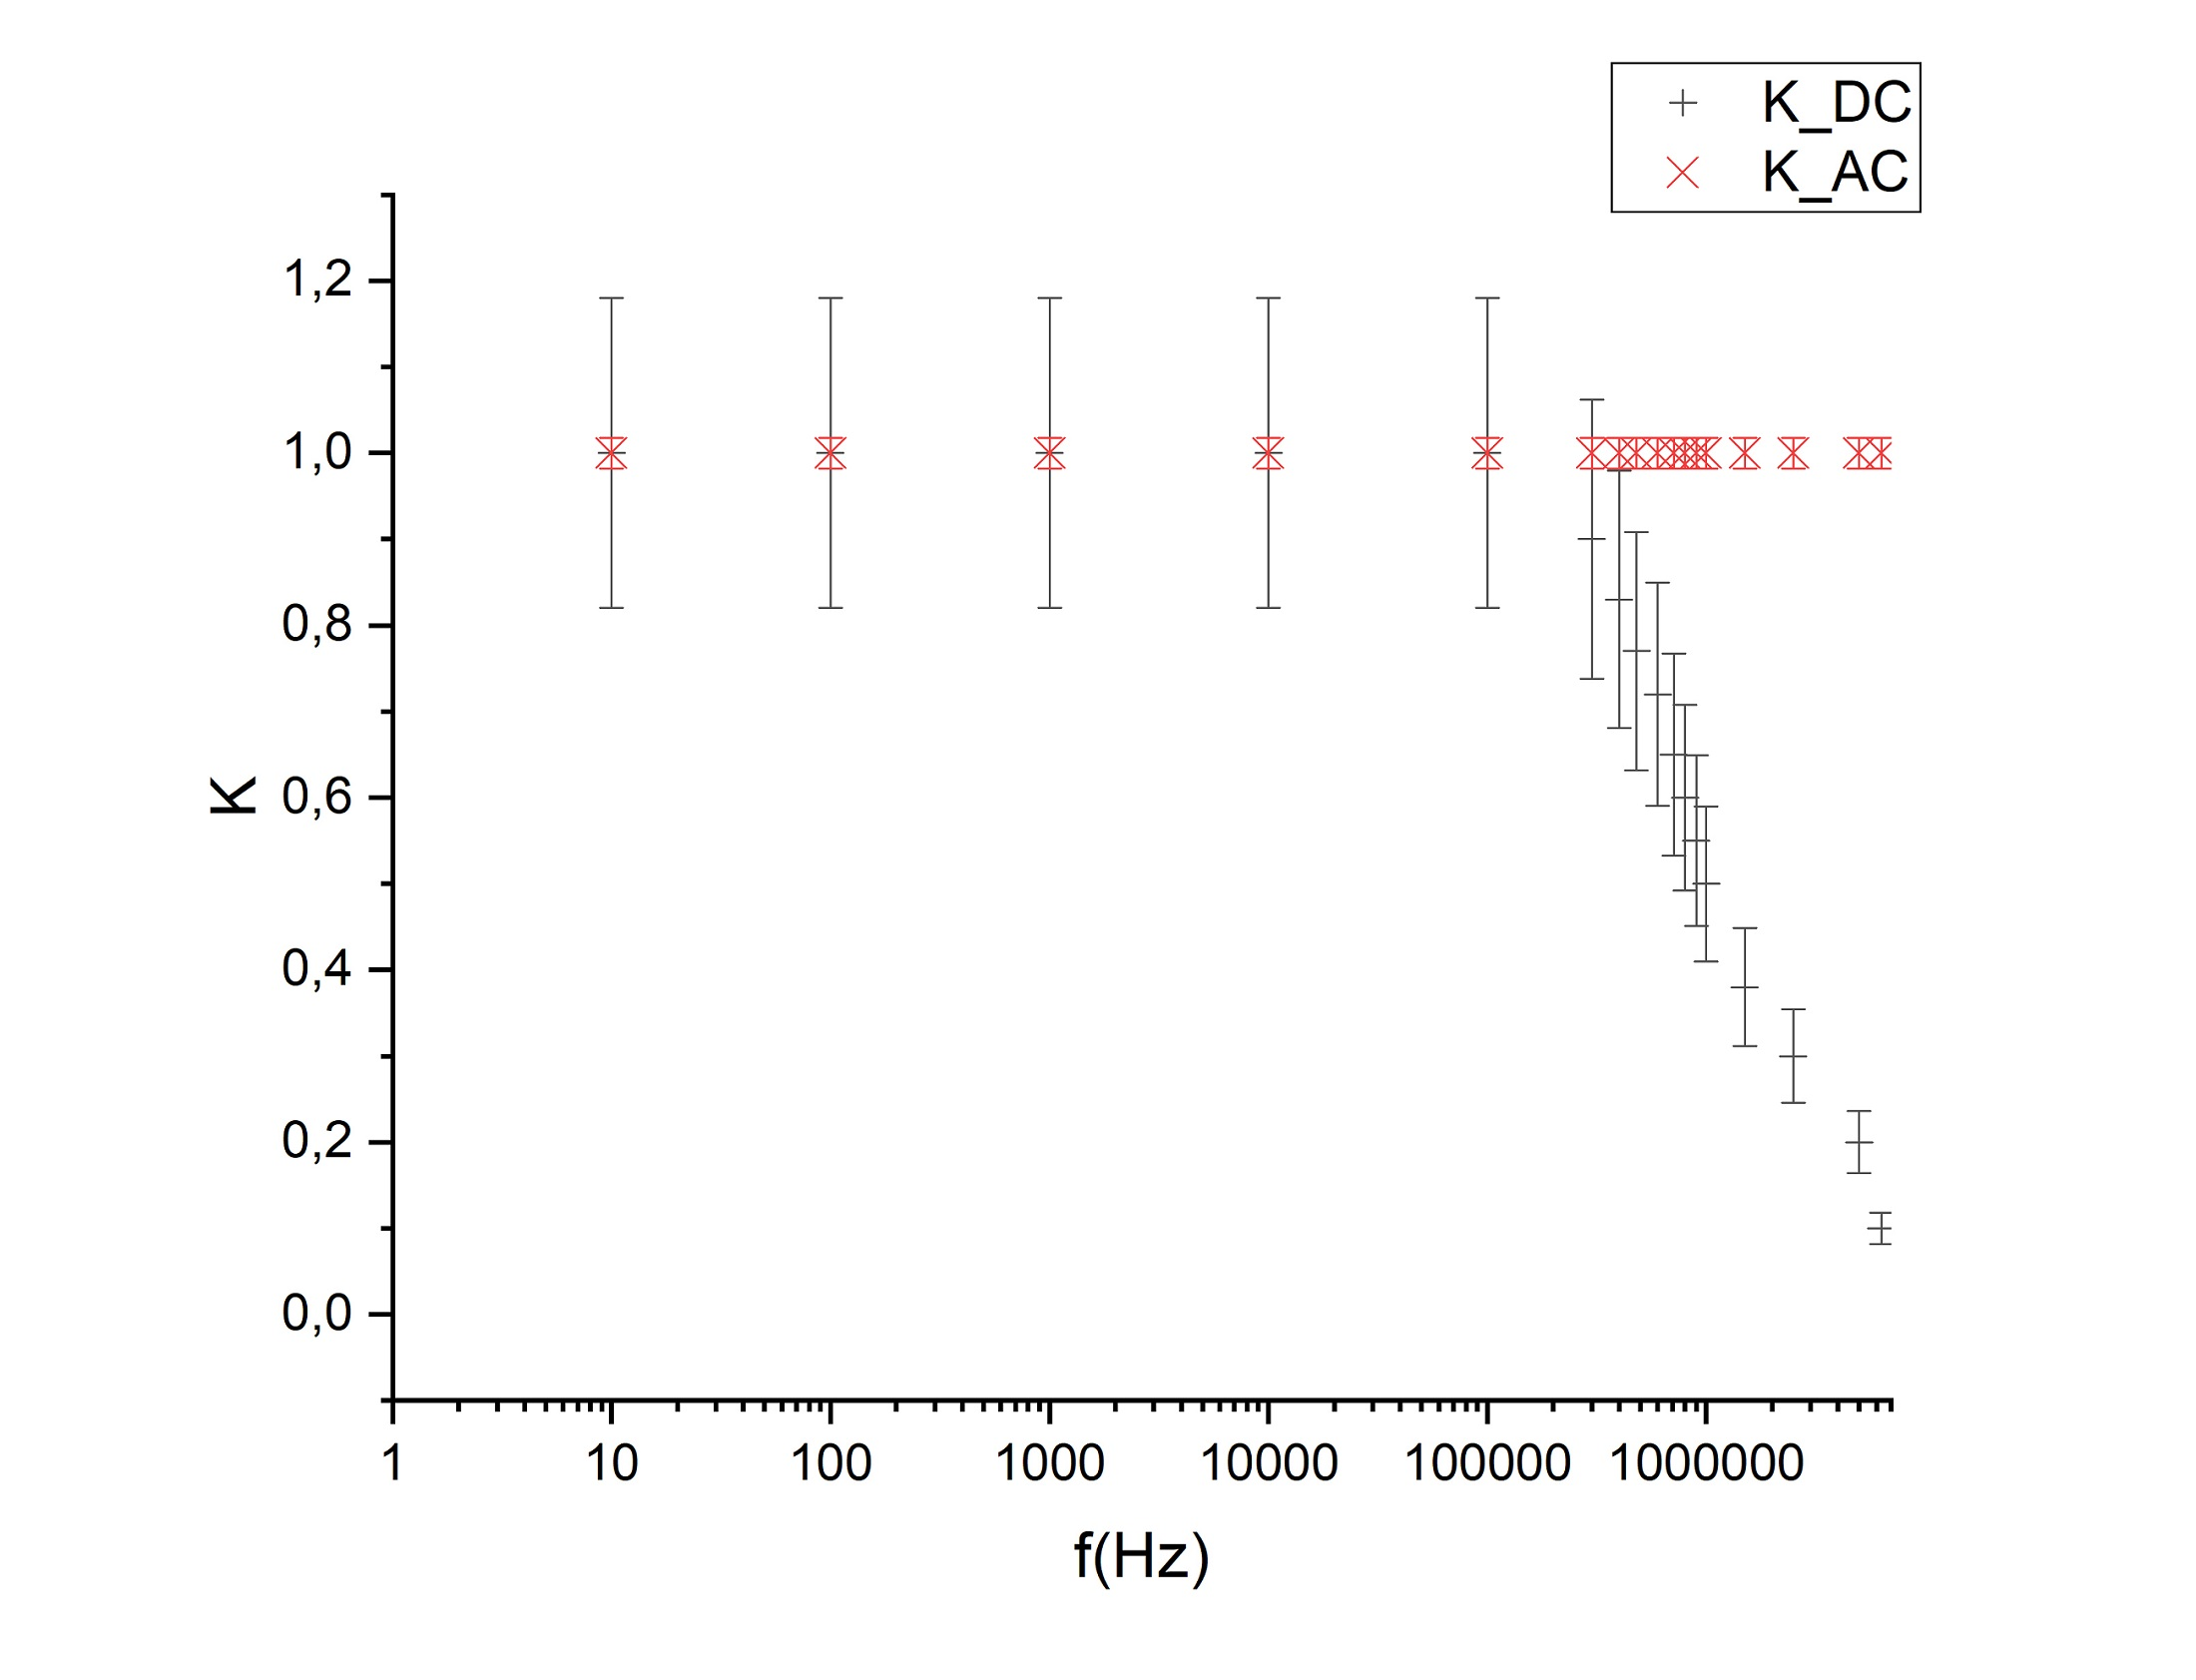
\includegraphics[]{116_23.jpg} \\
	\end{enumerate}
	\item \textbf{Изучение влияния АЧХ на искажение сигнала.} Устанавливаем на генераторе переключатель вида сигнала в положение "п" — прямоугольные импульсы (меандр). Получаем на экране устойчивую картину прямоугольных импульсов на частоте $f = 1 kHz$. Изменяя частоту генератора во всём диапазоне, наблюдаем как меняется вид отображаемого на осциллографе сигнала для открытого (DC) и закрытого (AC) входов канала CH2(Y). При изменении частоты используем ручку осциллографа TIME/DIV для регулировки масштаба по горизонтали (по времени). Запечатлеем характерный вид полученных осциллограмм для частот $f$, при которых форма прямоугольных импульсов существенно искажается.\\
	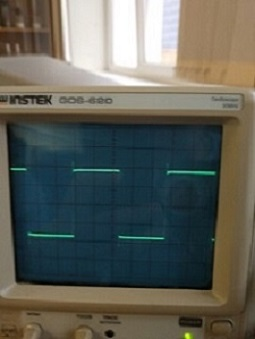
\includegraphics[]{116_1.jpg}
	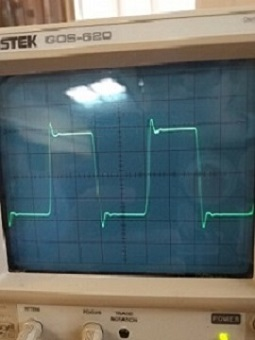
\includegraphics[]{116_3.jpg}\\
	Из-за эффекта Гиббса. \\
	Рассмотрим явление Гиббса на частном случае разрывной функции\\
	\[f(t) = sgn(t)\]
	Функция (1) является нечётной, поэтому её разложение в ряд Фурье будет содержать только синусы:
	\[f(t) = \sum_{m = 1}^{\infty}b_m sin(mt)\]
	где коэффициенты разложения $b_m$ определяются выражениями
	\[b_m = \dfrac{1}{\pi} \int_{- \pi}^{\pi} f(t) sin (mt) dt = \dfrac{2}{\pi} \int_0^{\pi} sin (mt) dt = \dfrac{2}{\pi m} (1-(-1)^m)m \]
	т. е. в разложении отличны от нуля только члены с нечётными номерами $m = 2n - 1$ и, следовательно, разложение в ряд Фурье приводится к виду
	\[f(t) = lim_{N \longrightarrow \infty} \left(\dfrac{4}{\pi} \sum_{n = 1}^N \dfrac{sin(2n-1)t}{2n-1} \right)\]
	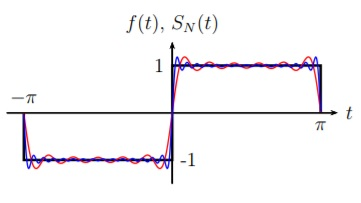
\includegraphics[]{116_21.jpg} \\
	Или из-за того, что на высоких частотах наблюдается отклонение амплитудного напряжения от 0, хотя при изменении частоты сигнала оно меняться не должно. 
	\item \textbf{Измерение разности фазово-частотных характеристик каналов осциллографа.}\\ Фазово-частотной характеристикой (ФЧХ) называют зависимость разности фаз входного и выходного сигналов от частоты. Осциллограф может быть использован для измерения разности фаз между подаваемыми на него сигналами, при этом однако необходимо учитывать, что каналы X и Y могут иметь разные ФЧХ. В данном пункте предлагается провести измерение разности фаз, возникающей при подаче одного и того же сигнала на разные каналы осциллографа, в зависимости от частоты сигнала.
	\begin{enumerate}
		\item Подайте синусоидальный сигнал частоты $f = 1 kHz$ с выхода звукового генератора через тройник (разветвитель) на каналы CH1(X) и преподавателя CH2(Y). Выключите внутреннюю развертку осциллографа, переведя переключатель TIME/DIV в положение X–Y. В этом режиме отклонение луча на экране пропорционально подаваемым на каналы напряжениям $ Y(t) =  k_yU_y(t), X(t) = k_xU_x(t)$, где коэффициенты масштаба $k_x$, $k_y$ определяются положениями ручек VOLTS/DIV.
		\item Установите переключатели режимов каналов X и Y в положение GND (выключены) и ручками POSITION установите точку в центр экрана. После этого установите переключатели режимов каналов X и Y в положения AC (закрытые входы). Используя ручки VOLTS/DIV обоих каналов, получите на экране отрезок прямой (вырожденный эллипс) под углом 45 градусов к горизонтали, занимающий большую часть экрана.\\
		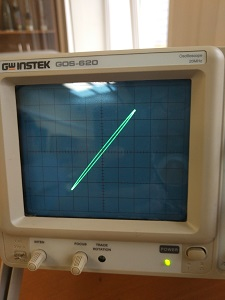
\includegraphics[]{116_6.jpg}\\
		\item Изменяя частоту генератора $f$ во всем доступном диапазоне найдите участки, на которых изображение на экране переходит из отрезка в невырожденный эллипс. На этих участках проведите подробное измерение разности фаз $\Delta \varphi (f)$ между каналами X и Y в зависимости от частоты. 
		\item Результаты измерений занесем в таблицу.
		\begin{figure} [h]
	\center{
	\begin{tabular}{|c|c|c|c|c|c|c|c|}
	\hline
	$f, Hz$&10&50&100&1000&10000&100000&10000000\\
	\hline
	$\Delta \varphi$, рад&0,93&0,34&0,17&0&0&0,08&0,22\\
	\hline
	\end{tabular}
	}
	\end{figure}\\
	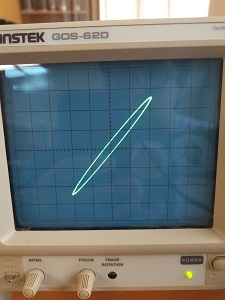
\includegraphics[]{116_12.jpg}
	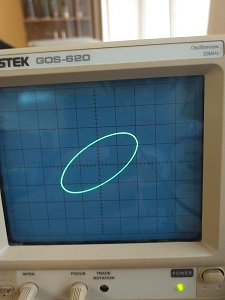
\includegraphics[]{116_10.jpg}\\
	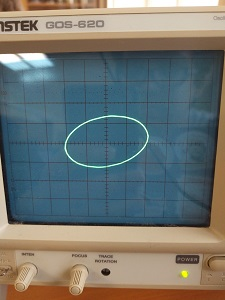
\includegraphics[]{116_8.jpg}
	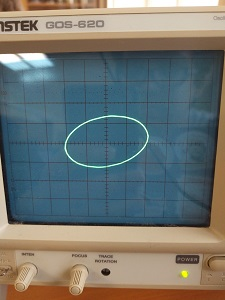
\includegraphics[]{116_8.jpg}\\
	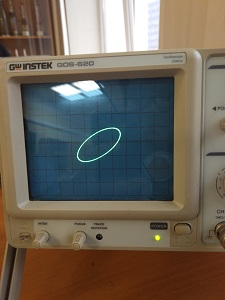
\includegraphics[]{116_5.jpg}
	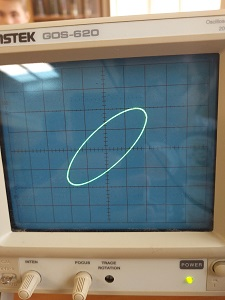
\includegraphics[]{116_9.jpg} \\
	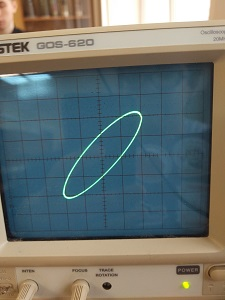
\includegraphics[]{116_14.jpg}\\
	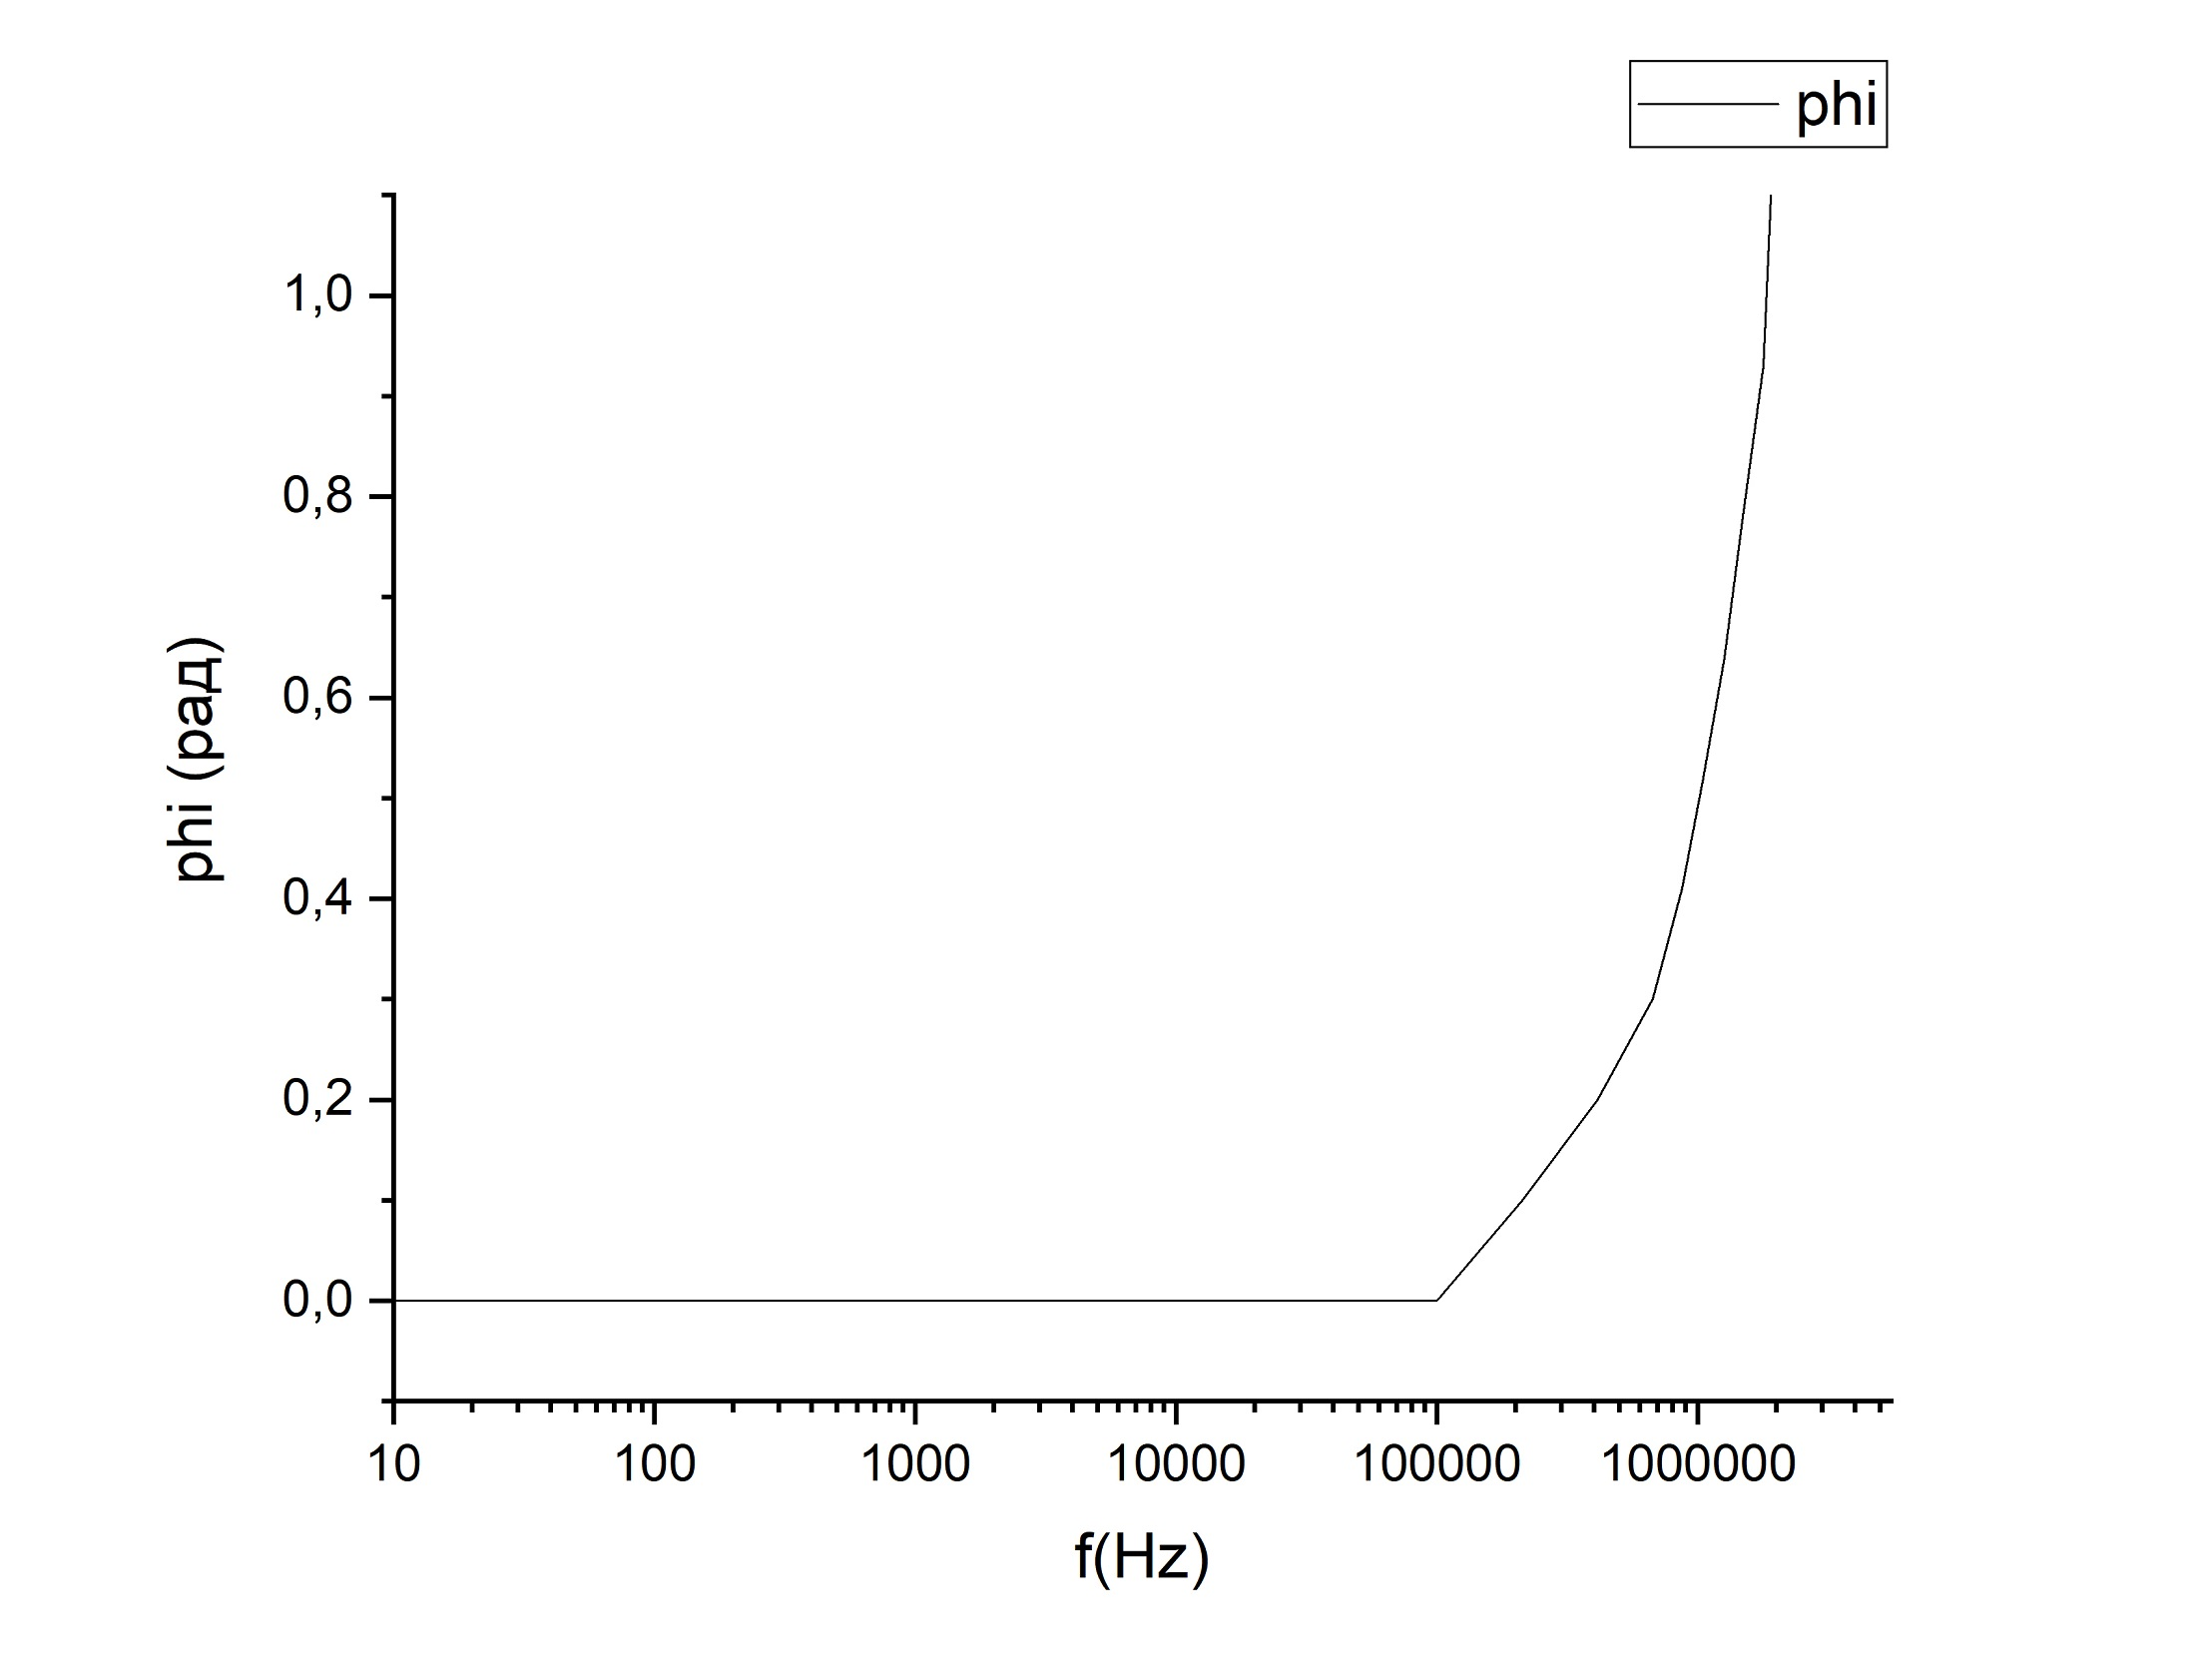
\includegraphics[]{116_24.jpg} \\
	\end{enumerate}
	При подаче на взаимно перпендикулярные отклоняющие пластины двух синусоидальных сигналов траектория луча на экране осциллографа представляет собой эллипс и может быть в общем виде описана уравнениями
	\[x(t) = A_x sin(\omega t + \varphi_x),\text{ } y(t) = A_y sin(\omega t + \varphi_y) \]
	\[\omega t = -\varphi_x\]
	\[|\Delta \varphi| = arcsin \vert \dfrac{y_o}{A_y} \vert \]
	или
	\[|\Delta \varphi| = \pi - arcsin \vert \dfrac{y_o}{A_y} \vert \]
\item \textbf{Наблюдение фигур Лиссажу и измерение частоты.} \\
\begin{enumerate}
\item Выключите внутреннюю развертку осциллографа (TIME/DIV в положение X-Y). Подайте на вход каналов X и Y осциллографа сигналы с двух разных звуковых генераторов. Установите приблизительно одинаковые частоты генераторов (рекомендуется использовать невысокие частоты $f \sim 50 \div 100$ Гц). Амплитуды генераторов положения ручек VOLTS/DIV осциллографа установите таким образом, чтобы фигура Лиссажу занимала большую часть экрана, не выходя за его пределы.
\item Изменяя $fx$, получите устойчивые фигуры для нескольких целочисленных отношений частот, например: $f_y / f_x$ = \\
1 : 1; 2 : 1;\\
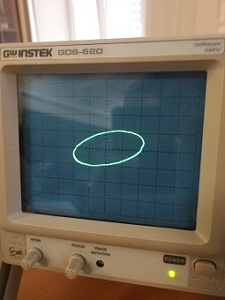
\includegraphics[]{116_17.jpg}
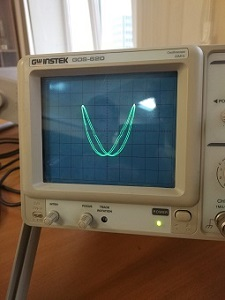
\includegraphics[]{116_18.jpg}\\
\newpage
 3 : 1; 3 : 2.\\
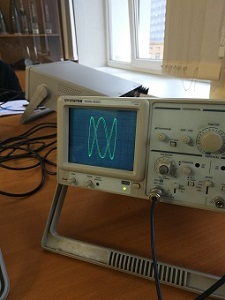
\includegraphics[]{116_19.jpg}
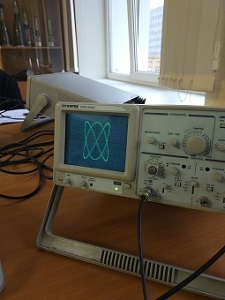
\includegraphics[]{116_20.jpg}
\end{enumerate}
\item
\textbf{Измерение АЧХ интегрирующей и дифференцирующей
RC-цепочек.} \\
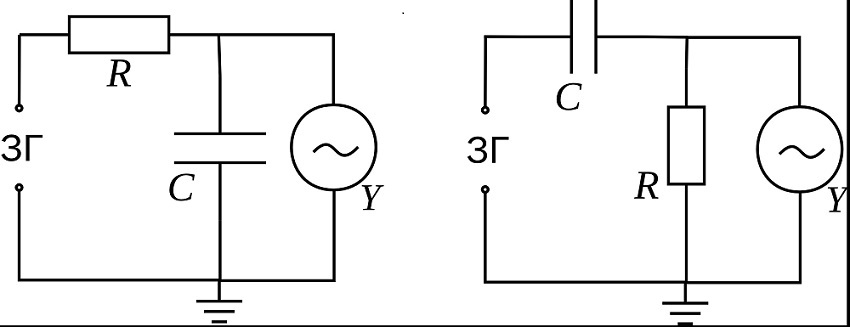
\includegraphics[]{116_22.jpg} \\
\[K_a(f) = \dfrac{1}{\sqrt{(\omega \tau)^2 + 1}} \]
\[K_b(f) = \dfrac{1}{\sqrt{(\omega \tau)^{-2} + 1}} \]
где $\tau = RC = 3*10^{-5} c$, $\omega = 2 \pi f$.\\
При проверке для $f = 5kHz$ $K \approx 0,7$ для обоих цепочек (проверено).
\newpage
Интегрирующая(a)
\begin{figure}[h]
\center{
\begin{tabular}{|c|c|c|c|c|c|c|c|}
\hline
$f, Hz$&101&1041&5042&10055&20000&50417&201050 \\
\hline
$\sigma_f, Hz$&1&1&1&1&1&1&1\\
\hline
$K$&1&1&0,7&0,47&0,25&0,1&0,032\\
\hline
$k_theor$&1&0,98&0,72&0,45&0,26&0,1&0,026\\
\hline
$sigma_K$&0,044&0,14&0,14&0,044&0,044&0,044&0,04\\
\hline
\end{tabular}
}
\end{figure}\\
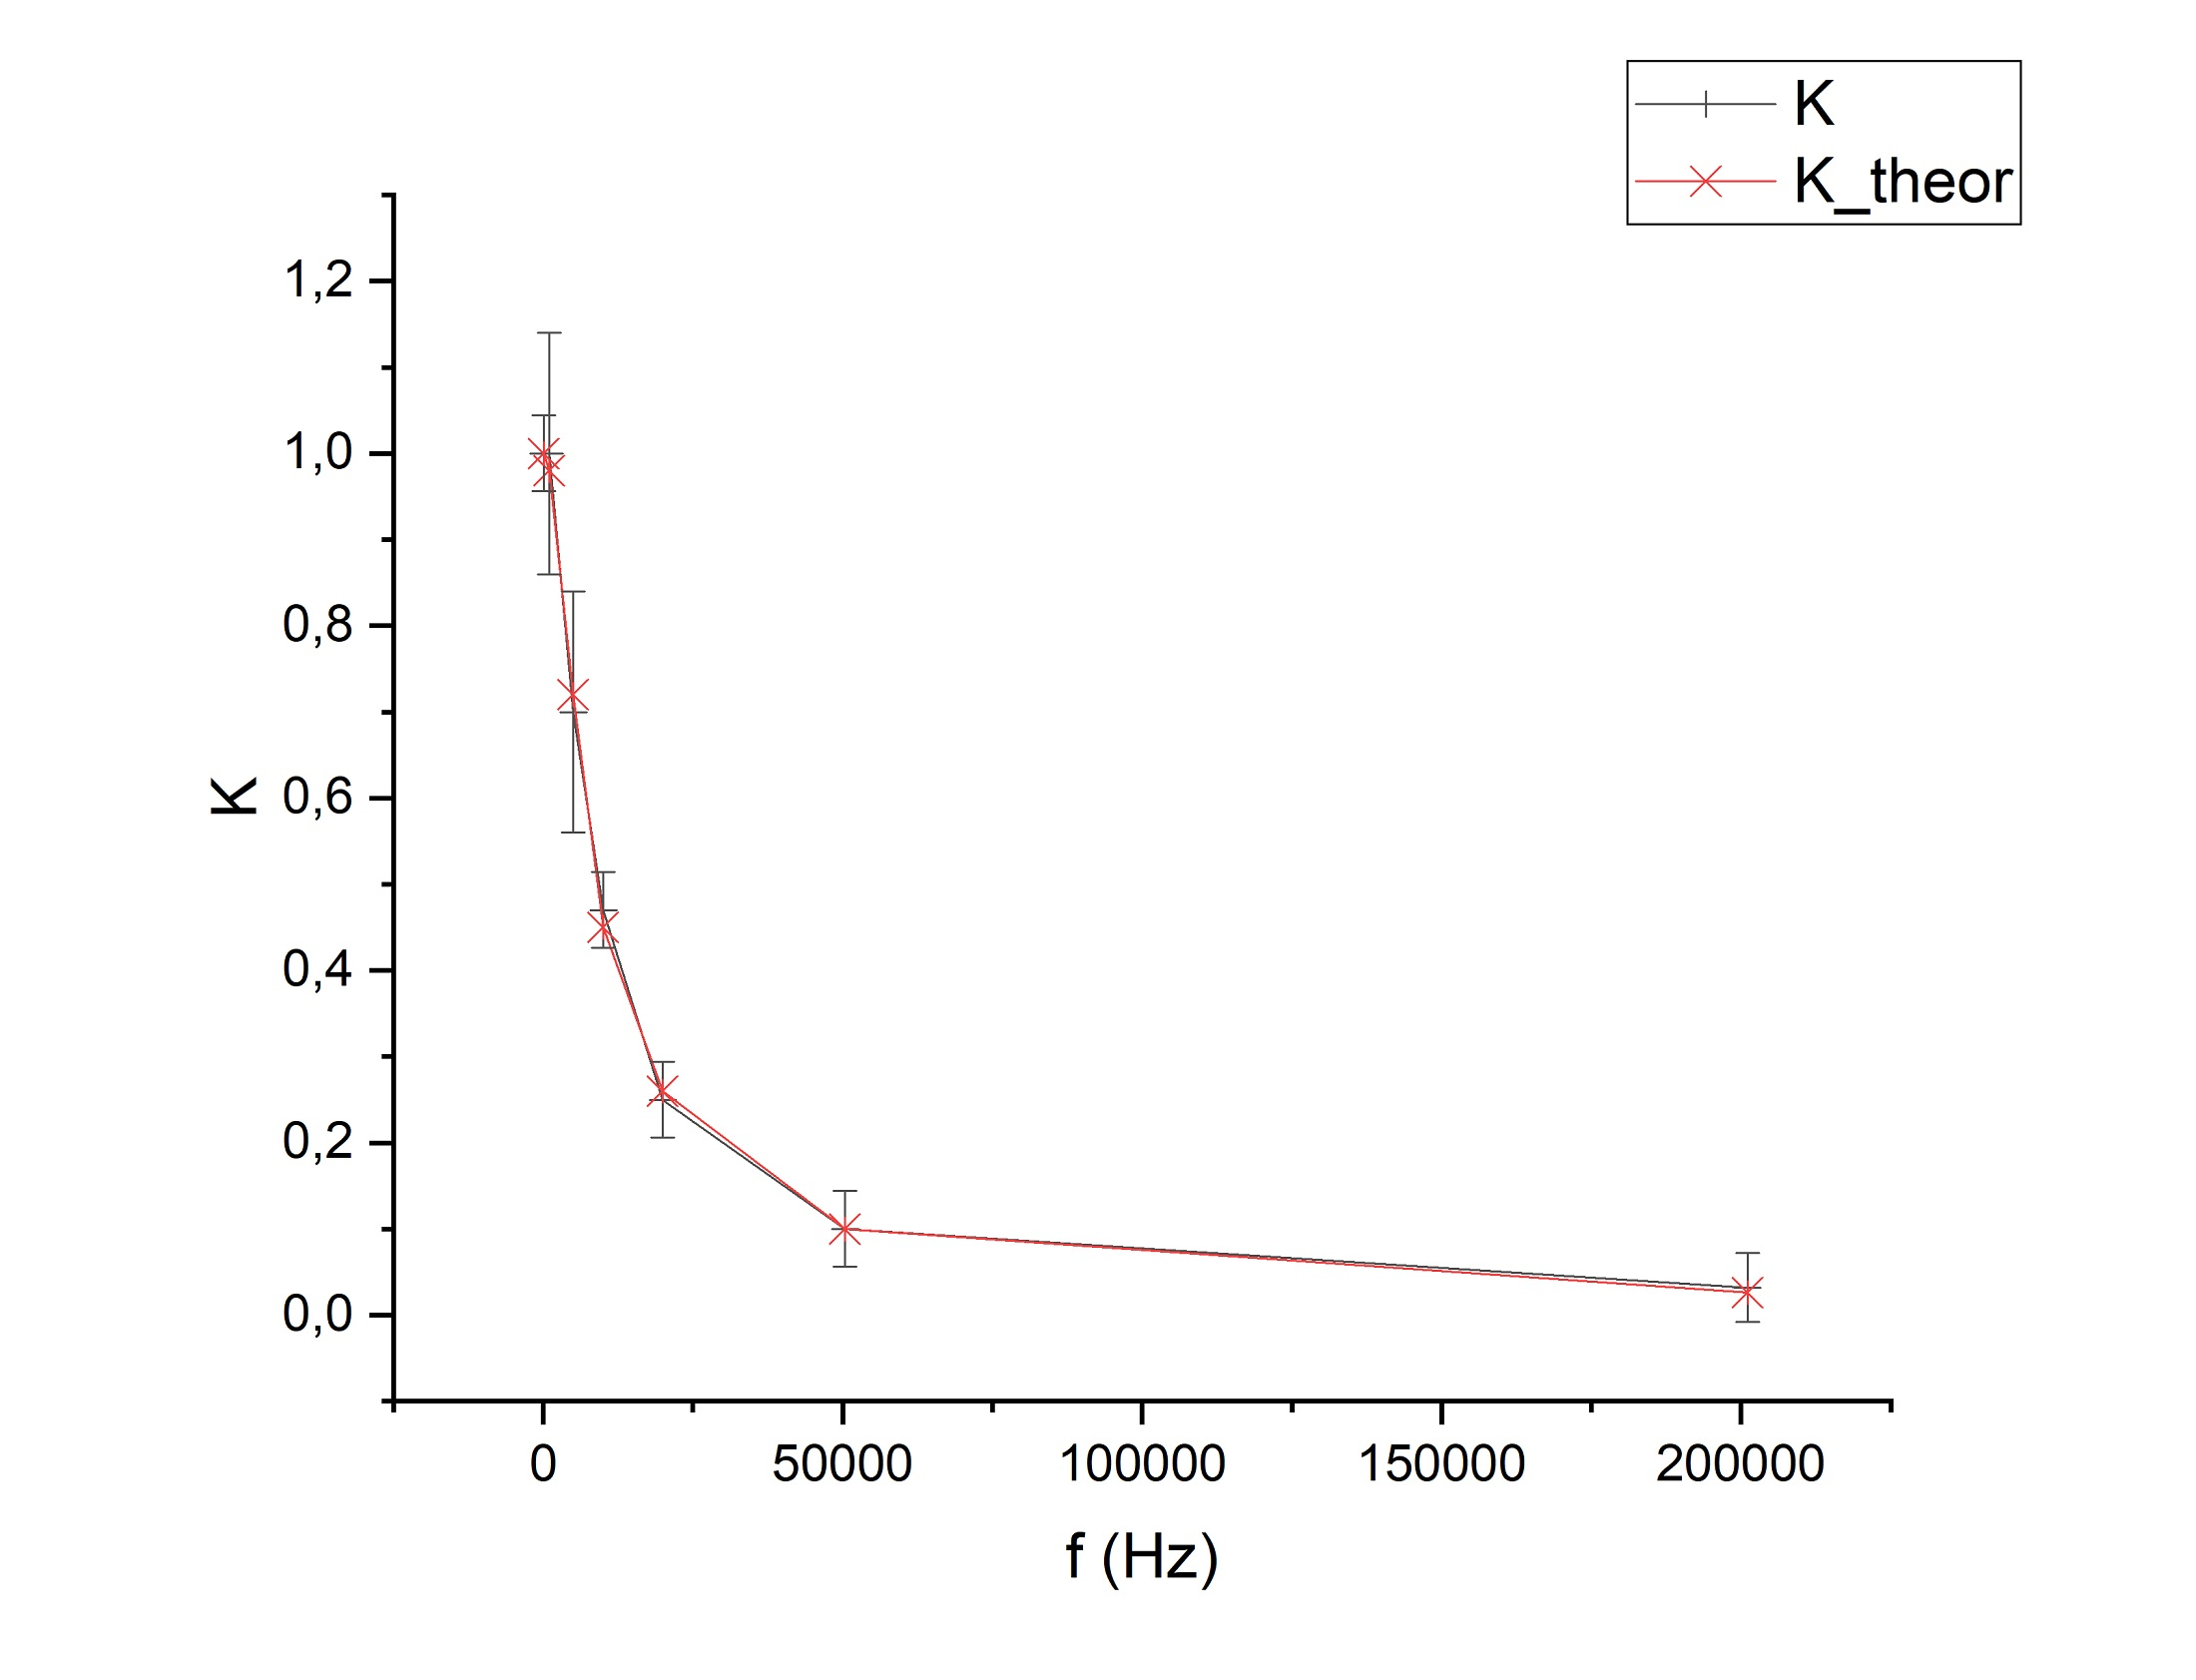
\includegraphics[]{116_25.jpg}\\
\newpage
Дифферинцирующая (b)
\begin{figure}[h]
\center{
\begin{tabular}{|c|c|c|c|c|c|c|c|}
\hline
$f, Hz$&101&1008&5007&10440&20132&50060&201340 \\
\hline
$\sigma_f, Hz$&1&1&1&1&1&1&1\\
\hline
$K$&0,2&0,2&0,7&0,9&0,95&1&1\\
\hline
$k_theor$&0,18&0,19&0,69&0,89&0,97&0,99&1\\
\hline
$sigma_K$&0,14&0,14&0,044&0,044&0,04&0,14&0,14\\
\hline
\end{tabular}
}
\end{figure} \\
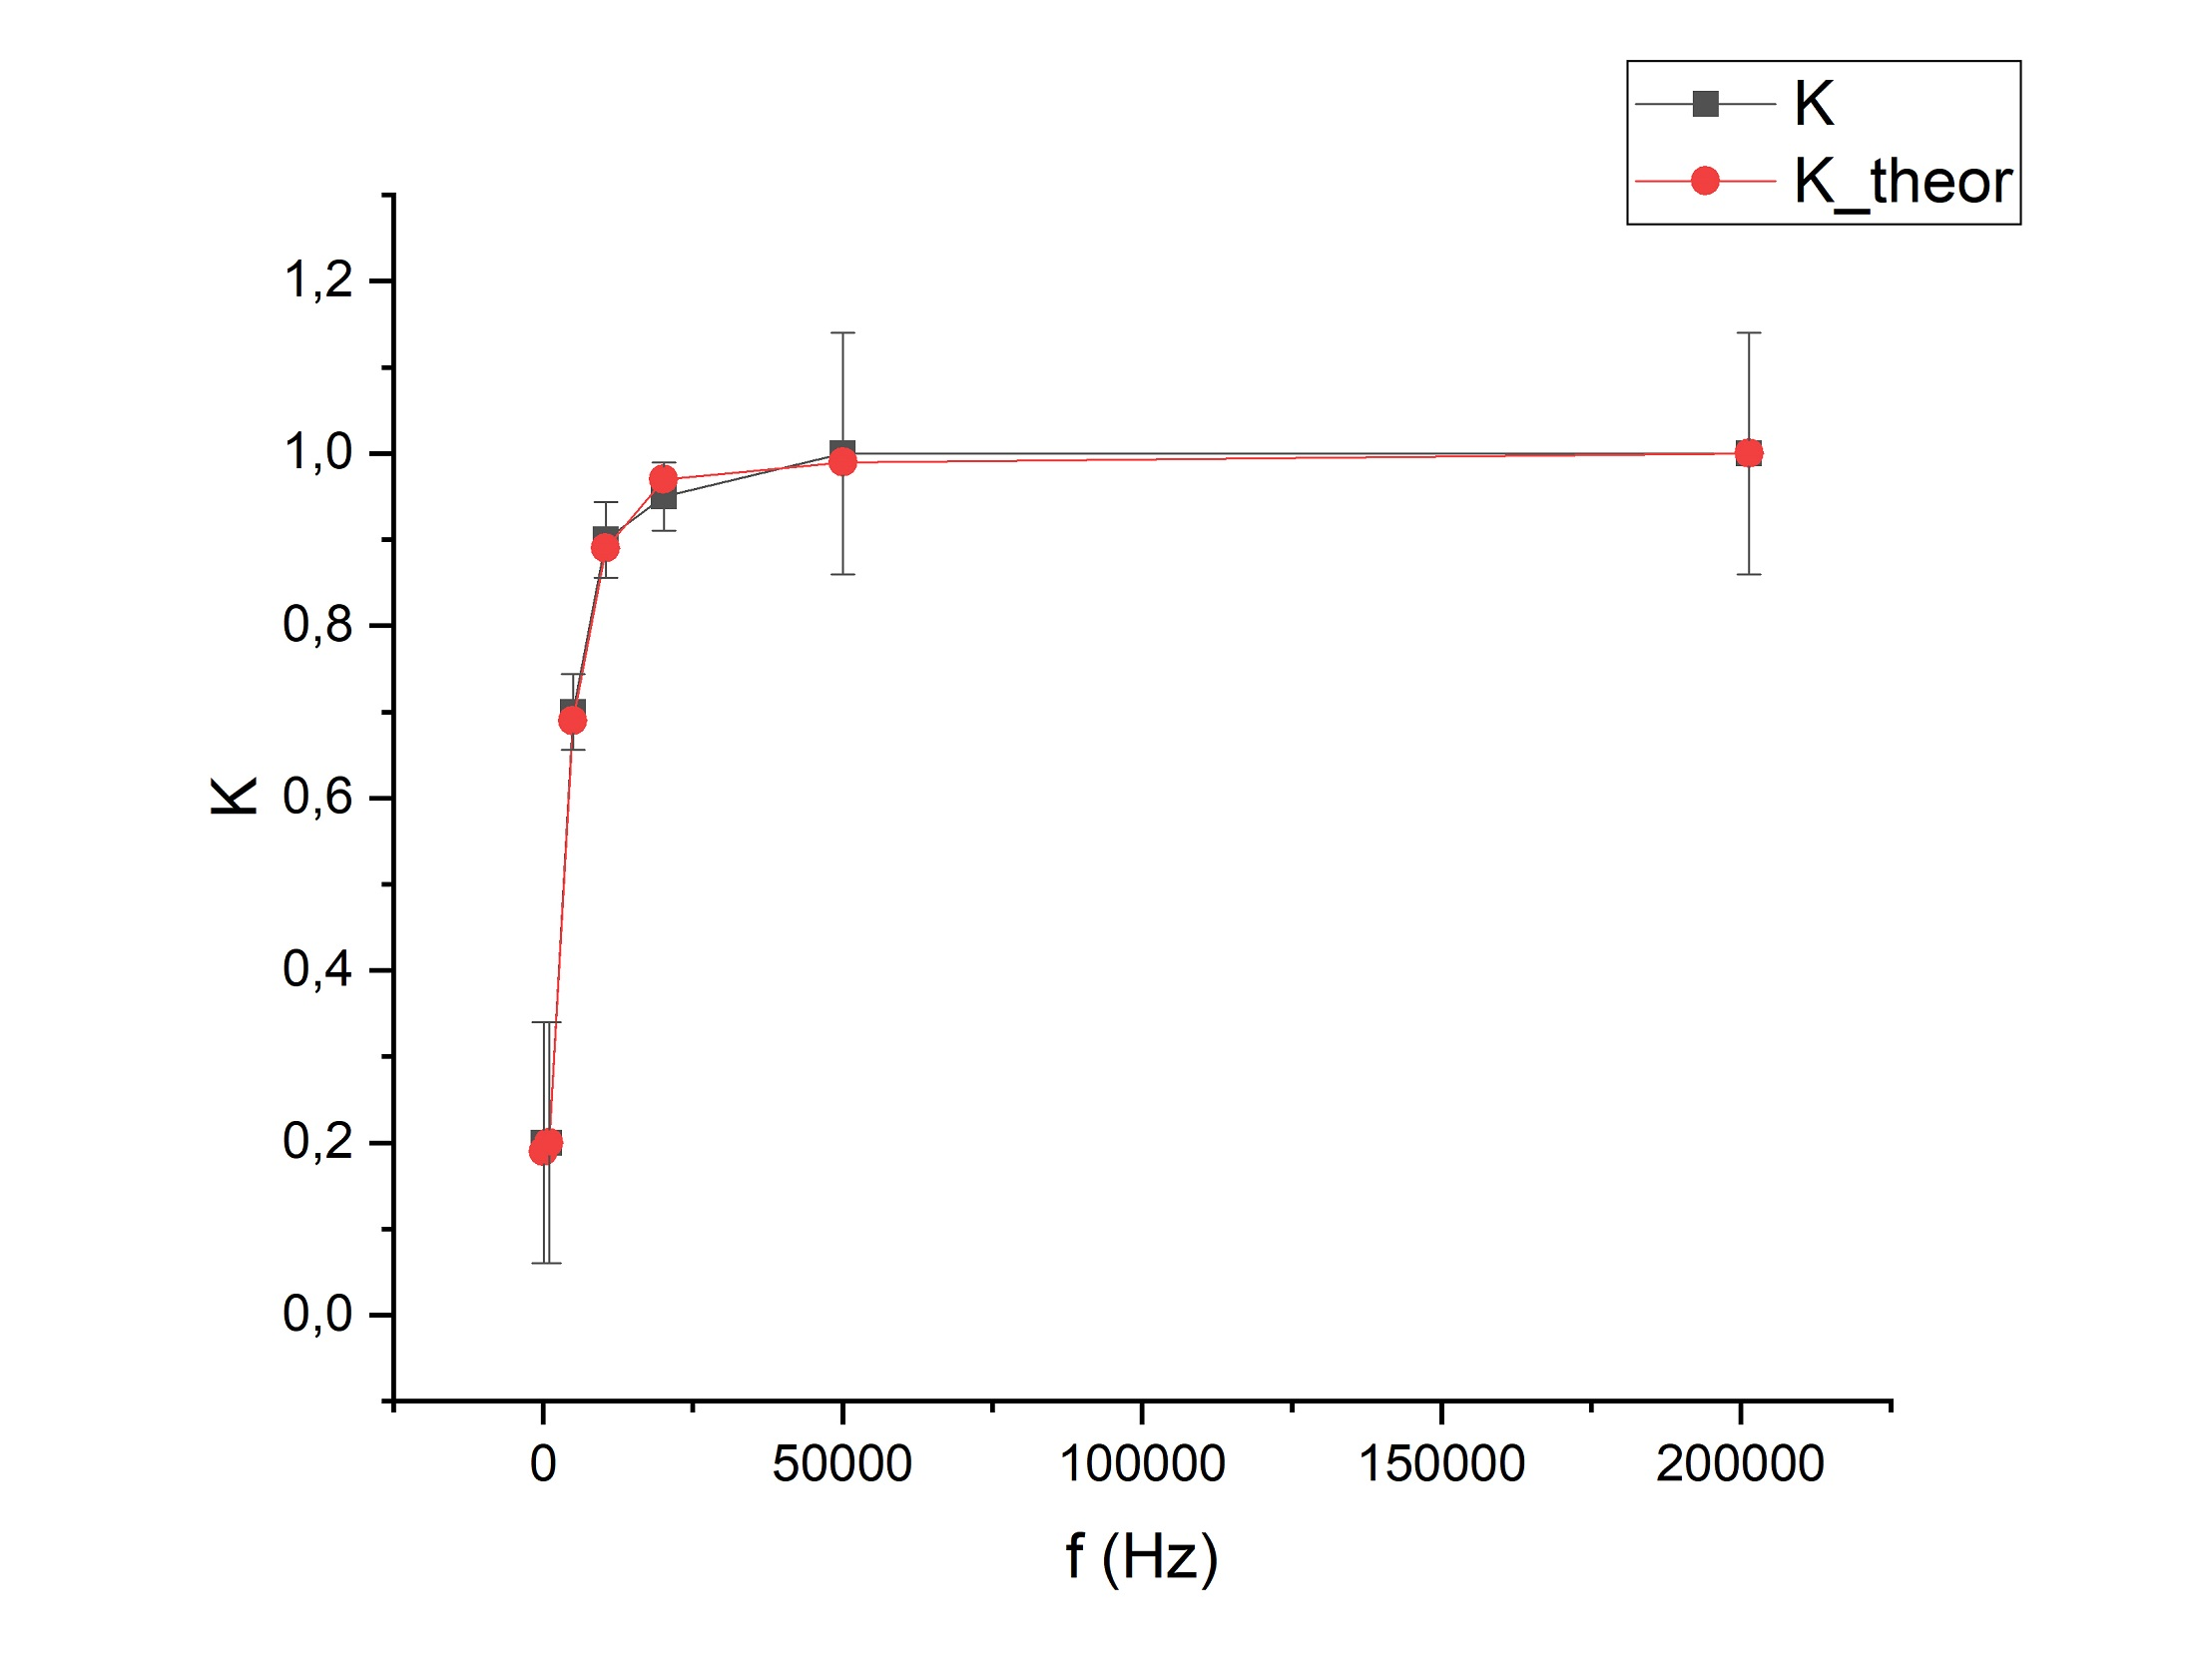
\includegraphics[]{116_26.jpg}\\
\end{enumerate}
\end{document}